\section{Запись СЛАУ}

Перейдём к одноиндексной записи

\[
  m = j(N_r + 1) + i
\]

Индексы изменяются в следующих границах:
\[
  0 \leq i \leq N_r
\]

\[
  0 \leq j \leq N_z
\]

Тогда имеем:
\[
  0 \leq m < (N_r + 1)(N_y + 1)
\]

\subsection{Запись для внутренних точек}
Перепишем наше уравнение с использованием нового индеса для $ i \in (0, N_r)$ и $ j \in (0, N_z) $:

\begin{align*}
  &- \left [ 
  h_z r_{i+\frac{1}{2}} k_1(r_{i+\frac{1}{2}}, z_j) \frac{v_{i+1, j} - v_{i, j}}{h_{r}}
  - h_z r_{i-\frac{1}{2}} k_1(r_{i-\frac{1}{2}}, z_j) \frac{v_{i, j} - v_{i - 1, j}}{h_{r}}
  \right . \\
  &\left .
  + h_r r_{i} k_2(r_i, z_{j+\frac{1}{2}}) \frac{v_{i, j + 1} - v_{i, j}}{h_{z}}
  - h_r r_{i} k_2(r_i, z_{j-\frac{1}{2}}) \frac{v_{i, j} - v_{i, j - 1}}{h_z}
  \right ]  = h_r h_z r_i f_{i, j}
\end{align*}

\begin{align*}
  & -\frac{h_r}{h_z} r_i k_2(r_i, z_{j - \frac{1}{2}}) v_{i, j - 1} - \frac{h_z}{h_r} r_{i - \frac{1}{2}} k_1(r_{i - \frac{1}{2}}, z_j) v_{i - 1, j} + \\
  & + \left[ 
    \frac{h_z}{h_r} r_{i + \frac{1}{2}} k_1(r_{i + \frac{1}{2}}, z_j) + \frac{h_z}{h_r} r_{i - \frac{1}{2}} k_1(r_{i - \frac{1}{2}}, z_j) +
    \frac{h_r}{h_z} r_i k_2 (r_i, z_{j + \frac{1}{2}}) + \frac{h_r}{h_z} r_i k_2 (r_i, z_{j-\frac{1}{2}})
   \right] v_{i, j} \\
  & - \frac{h_z}{h_r} r_{i + \frac{1}{2}} k_1(r_{i+ \frac{1}{2}}, z_j) v_{i + 1, j} - \frac{h_r}{h_z} r_i k_2(r_i, z_{j + 1}) v_{i, j + \frac{1}{2}}
  = h_r h_z r_i f_{i, j}
\end{align*}

Введём новые обозначения:

\[
  a_m w_{m - L} + b_m w_{m - 1} + c_m w_m + d_m w_{m + 1} + e_m w_{m + L} = g_m
\]

где коэффициенты равны:
\[
  a_m = -\frac{h_r}{h_z} r_i k_2(r_i, z_{j - \frac{1}{2}})
\]

\[
  b_m = - \frac{h_z}{h_r} r_{i - \frac{1}{2}} k_1(r_{i - \frac{1}{2}}, z_j)
\]

\[
  c_m = \frac{h_z}{h_r} r_{i + \frac{1}{2}} k_1(r_{i + \frac{1}{2}}, z_j) + \frac{h_z}{h_r} r_{i - \frac{1}{2}} k_1(r_{i - \frac{1}{2}}, z_j) +
  \frac{h_r}{h_z} r_i k_2 (r_i, z_{j + \frac{1}{2}}) + \frac{h_r}{h_z} r_i k_2 (r_i, z_{j-\frac{1}{2}})
\]

\[
  d_m = - \frac{h_z}{h_r} r_{i + \frac{1}{2}} k_1(r_{i+ \frac{1}{2}}, z_j)
\]

\[
  e_m = - \frac{h_r}{h_z} r_i k_2(r_i, z_{j + \frac{1}{2}})
\]

\[
  g_m = h_r h_z r_i f_{i, j}
\]

\subsection{Запись для левой границы}

Перепишем наше уравнение с использованием нового индекса для $i = 0$ и $ j \in (0, N_z) $:

\begin{align*}
  &- \left [ 
    h_z r_{\frac{1}{2}} k_1(r_{\frac{1}{2}}, z_j) \frac{v_{1, j} - v_{0, j}}{h_{r}}
    - 0
    \right . \\
    &\left .
    + \frac{h_r}{2} \frac{r_{\frac{1}{2}}}{2} k_2(r_0, z_{j+\frac{1}{2}}) \frac{v_{0, j + 1} - v_{0, j}}{h_{z}}
    - \frac{h_r}{2} \frac{r_{\frac{1}{2}}}{2} k_2(r_0, z_{j-\frac{1}{2}}) \frac{v_{0, j} - v_{0, j - 1}}{h_z}
    \right ]  = \frac{h_r}{2} \frac{r_{\frac{1}{2}}}{2} h_z f_{0, j}
\end{align*}

\begin{align*}
  & - \frac{h_r}{2 h_z} \frac{r_{\frac{1}{2}}}{2} k_2(r_0, z_{j - \frac{1}{2}}) v_{0, j - 1} + \\
  & + \left[
    \frac{h_z}{h_r} r_{\frac{1}{2}} k_1(r_{\frac{1}{2}}, z_j) + \frac{h_r}{2 h_z} \frac{r_{\frac{1}{2}}}{2} k_2(r_0, z_{j+\frac{1}{2}})
    + \frac{h_r}{2 h_z} \frac{r_{\frac{1}{2}}}{2} k_2(r_0, z_{j -\frac{1}{2}})
  \right] v_{0, j} \\
  & - \frac{h_z}{h_r} r_{\frac{1}{2}} k_1(r_{\frac{1}{2}}, z_j) v_{1, j}
  - \frac{h_r}{2 h_z} \frac{r_{\frac{1}{2}}}{2} k_2(r_0, z_{j + \frac{1}{2}}) v_{0, j + 1} = \frac{h_r}{2} \frac{r_{\frac{1}{2}}}{2} h_z f_{0, j}
\end{align*}

Введём новые обозначения:

\[
  a_m w_{m - L} + c_m w_m + d_m w_{m + 1} + e_m w_{m + L} = g_m
\]

где коэффициенты равны:

\[
  a_m = - \frac{h_r}{2 h_z} \frac{r_{\frac{1}{2}}}{2} k_2(r_0, z_{j - \frac{1}{2}})
\]

\[
  c_m = \frac{h_z}{h_r} r_{\frac{1}{2}} k_1(r_{\frac{1}{2}}, z_j) + \frac{h_r}{2 h_z} \frac{r_{\frac{1}{2}}}{2} k_2(r_0, z_{j+\frac{1}{2}})
  + \frac{h_r}{2 h_z} \frac{r_{\frac{1}{2}}}{2} k_2(r_0, z_{j -\frac{1}{2}})
\]

\[
  d_m = - \frac{h_z}{h_r} r_{\frac{1}{2}} k_1(r_{\frac{1}{2}}, z_j)
\]

\[
  e_m = - \frac{h_r}{2 h_z} \frac{r_{\frac{1}{2}}}{2} k_2(r_0, z_{j + \frac{1}{2}})
\]

\[
  g_m = \frac{h_r}{2} \frac{r_{\frac{1}{2}}}{2} h_z f_{0, j}
\]

\subsection{Запись для правой границы}
Перепишем наше уравнение с использованием нового индекса для $i = N_r$ и $ j \in (0, N_z) $:

\begin{align*}
  &- \left [ 
  -h_z r_{N_r} ( \chi_2 v_{N_r, j} - \varphi_2(z))
  - h_z r_{N_r-\frac{1}{2}} k_1(r_{N_r-\frac{1}{2}}, z_j) \frac{v_{N_r, j} - v_{N_r - 1, j}}{h_{r}}
  \right . \\
  &\left .
  + \frac{h_r}{2} r_{N_r} k_2(r_{N_r}, z_{j+\frac{1}{2}}) \frac{v_{N_r, j + 1} - v_{N_r, j}}{h_{z}}
  - \frac{h_r}{2} r_{N_r} k_2(r_{N_r}, z_{j-\frac{1}{2}}) \frac{v_{N_r, j} - v_{N_r, j - 1}}{h_z}
  \right ]  = \frac{h_r}{2} r_{N_r} h_z f_{N_r, j}
\end{align*}

\begin{align*}
  & - \frac{h_r}{2h_z} r_{N_r} k_2(r_{N_r}, z_{j - \frac{1}{2}}) v_{N_r, j - 1}
  - \frac{h_z}{h_r} r_{N_r - \frac{1}{2}} k_1(r_{N_r - \frac{1}{2}}, z_j) v_{N_r - 1, j} \\
  & +\left[
    h_z r_{N_r} \chi_2  + \frac{h_z}{h_r} r_{N_r - \frac{1}{2}} k_1(r_{N_r -\frac{1}{2}}, z_j)
    + \frac{h_r}{2 h_z} r_{N_r} k_2(r_{N_r, z_{j + \frac{1}{2}}})
    + \frac{h_r}{2 h_z} r_{N_r} k_2 (r_{N_r}, z_{j - \frac{1}{2}})
  \right] v_{N_r, j} \\
  &- \frac{h_r}{2 h_z} r_{N_r} k_2(r_{N_r}, z_{j + \frac{1}{2}}) v_{N_r, j + 1}
  = \frac{h_r}{2} r_{N_r} h_z f_{N_r, j} + h_z r_{N_r} \varphi_2(z)
\end{align*}

Введём новые обозначения:
\[
  a_m w_{m - L} + b_m w_{m - 1} + c_m w_m + e_m w_{m + L} = g_m
\]

где коэффициенты:

\[
  a_m = - \frac{h_r}{2h_z} r_{N_r} k_2(r_{N_r}, z_{j - \frac{1}{2}})
\]

\[
  b_m = - \frac{h_z}{h_r} r_{N_r - \frac{1}{2}} k_1(r_{N_r - \frac{1}{2}}, z_j)
\]

\[
  c_m = h_z r_{N_r} \chi_2  + \frac{h_z}{h_r} r_{N_r - \frac{1}{2}} k_1(r_{N_r -\frac{1}{2}}, z_j)
  + \frac{h_r}{2 h_z} r_{N_r} k_2(r_{N_r, z_{j + \frac{1}{2}}})
  + \frac{h_r}{2 h_z} r_{N_r} k_2 (r_{N_r}, z_{j - \frac{1}{2}})
\]

\[
  e_m = - \frac{h_r}{2 h_z} r_{N_r} k_2(r_{N_r}, z_{j + \frac{1}{2}})
\]

\[
  g_m =\frac{h_r}{2} r_{N_r} h_z f_{N_r, j} + h_z r_{N_r} \varphi_2(z)
\]

\subsection{Запись для нижней границы}
Перепишем наше уравнение с использованием нового индекса для $i \in (0, N_r) $ и $ j = 0 $:

\begin{align*}
  - \left [ 
  \frac{h_z}{2} r_{i+\frac{1}{2}} k_1(r_{i+\frac{1}{2}}, z_0) \frac{v_{i+1, 0} - v_{i, 0}}{h_{r}}
  - \frac{h_z}{2} r_{i-\frac{1}{2}} k_1(r_{i-\frac{1}{2}}, z_0) \frac{v_{i, 0} - v_{i - 1, 0}}{h_{r}}
  \right . \\
  \left .
  + h_r r_{i} k_2(r_i, z_{\frac{1}{2}}) \frac{v_{i, 1} - v_{i, 0}}{h_{z}}
  - h_r r_i (\chi_3 v_{i, 0} - \varphi_3(r))
  \right ]  = h_r \frac{h_z}{2} r_i f_{i, 0}
\end{align*}

\begin{align*}
  &  - \frac{h_z}{2 h_r} v_{i - \frac{1}{2}} k_1(r_{i - \frac{1}{2}}, z_0) v_{i - 1, 0} \\
  & + \left[ 
    h_r r_i \chi_3 +\frac{h_z}{2 h_r} r_{i + \frac{1}{2}} k_1(r_{i + \frac{1}{2}}, z_0) + \frac{h_z}{2 h_r} r_{i - \frac{1}{2}} k_1(r_{i - \frac{1}{2}}, z_0)
    + \frac{h_r}{h_z} r_i k_2(r_i, z_{\frac{1}{2}}) 
  \right] v_{i, 0} \\
  & - \frac{h_z}{2 h_r} r_{i + \frac{1}{2}} k_1(r_{i + \frac{1}{2}}, z_0) v_{i + 1, 0} - \frac{h_r}{h_z} r_i k_2 (r_i, z_{\frac{1}{2}}) v_{i, 1}
  = h_r \frac{h_z}{2} r_i f_{i, 0} + h_r r_i \varphi(r)
\end{align*}

Введём новые обозначения:
\[
  b_m w_{m - 1} + c_m w_m + d_m w_{m + 1} + e_m w_{m + L} = g_m
\]

где коэффициенты ранвы:
\[
  b_m = - \frac{h_z}{2 h_r} r_{i - \frac{1}{2}} k_1(r_{i - \frac{1}{2}}, z_0)
\]

\[
  c_m = h_r r_i \chi_3 +\frac{h_z}{2 h_r} r_{i + \frac{1}{2}} k_1(r_{i + \frac{1}{2}}, z_0) + \frac{h_z}{2 h_r} r_{i - \frac{1}{2}} k_1(r_{i - \frac{1}{2}}, z_0)
  + \frac{h_r}{h_z} r_i k_2(r_i, z_{\frac{1}{2}}) 
\]

\[
  d_m = - \frac{h_z}{2 h_r} r_{i + \frac{1}{2}} k_1(r_{i + \frac{1}{2}}, z_0)
\]

\[
  e_m = - \frac{h_r}{h_z} r_i k_2 (r_i, z_{\frac{1}{2}})
\]

\[
  g_m = h_r \frac{h_z}{2} r_i f_{i, 0} + h_r r_i \varphi_3(r)
\]

\subsection{Запись для верхней границы}
Перепишем наше уравнение с использованием нового индекса для $i \in [0, N_r] $ и $ j = N_z $:

\[
  v_{i, N_z} = \varphi(r_i)
\]

Перейдём к новым обозначениям:
\[
  c_m w_m = \varphi_m
\]

где:
\[
  c_m = 1, \quad \varphi_m = \varphi_4(r_i)
\]


\subsection{Запись для левой нижней граничной точки}

Перепишем наше уравнение с использованием нового индекса для $i = 0 $ и $ j = 0 $:

\begin{align*}
  &- \left [ 
  \frac{h_z}{2} r_{\frac{1}{2}} k_1(r_{\frac{1}{2}}, z_0) \frac{v_{1, 0} - v_{0, 0}}{h_{r}}
  - 0
  \right . \\
  &\left .
  + \frac{h_r}{2} \frac{r_{\frac{1}{2}}}{2} k_2(r_0, z_{\frac{1}{2}}) \frac{v_{0, 1} - v_{0, 0}}{h_{z}}
  - \frac{h_r}{2} \frac{r_{\frac{1}{2}}}{2} (\chi_3 v_{0, 0} - \varphi_3(r))
  \right ]  = \frac{h_r}{2} \frac{h_z}{2} \frac{r_{\frac{1}{2}}}{2} f_{0, 0}
\end{align*}

\begin{align*}
  &\left[
    \frac{h_z}{2 h_r} r_{\frac{1}{2}} k_1(r_{\frac{1}{2}}, z_0) + \frac{h_r}{2 h_z} \frac{r_{\frac{1}{2}}}{2} k_2(r_0, z_{\frac{1}{2}}) + \frac{h_r}{2} \frac{r_\frac{1}{2}}{2} \chi_3
  \right] v_{0, 0} - \\
  & - \frac{h_z}{2 h_r} r_\frac{1}{2} k_1(r_\frac{1}{2}, z_0) v_{1,0} 
  - \frac{h_r}{2 h_z} \frac{r_{\frac{1}{2}}}{2} k_2(r_0, z_{\frac{1}{2}}) v_{0, 1}
  = \frac{h_r}{2} \frac{h_z}{2} \frac{r_{\frac{1}{2}}}{2} f_{0, 0} + \frac{h_r}{2} \frac{r_{\frac{1}{2}}}{2} \varphi_3(r_0)
\end{align*}

Введём новые обозначения:
\[
  c_m w_m + d_m w_{m + 1} + e_m w_{m + L} = g_m
\]

где коэффициенты ранвы:

\[
  c_m = \frac{h_z}{2 h_r} r_{\frac{1}{2}} k_1(r_{\frac{1}{2}}, z_0) + \frac{h_r}{2 h_z} \frac{r_{\frac{1}{2}}}{2} k_2(r_0, z_{\frac{1}{2}}) + \frac{h_r}{2} \frac{r_\frac{1}{2}}{2} \chi_3
\]

\[
  d_m = - \frac{h_z}{2 h_r} r_\frac{1}{2} k_1(r_\frac{1}{2}, z_0)
\]

\[
  e_m = - \frac{h_r}{2 h_z} \frac{r_{\frac{1}{2}}}{2} k_2(r_0, z_{\frac{1}{2}})
\]

\[
  g_m = \frac{h_r}{2} \frac{h_z}{2} \frac{r_{\frac{1}{2}}}{2} f_{0, 0} + \frac{h_r}{2} \frac{r_{\frac{1}{2}}}{2} \varphi_3(r_0)
\]

\subsection{Запись для правой нижней граничной точки}

Перепишем наше уравнение с использованием нового индекса для $i = N_r $ и $ j = 0 $:

\begin{align*}
  - \left [ 
  -\frac{h_z}{2} r_{N_r} (\chi_2 v_{N_r, 0} - \varphi_2(z) )
  - \frac{h_z}{2} r_{N_r-\frac{1}{2}} k_1(r_{N_r-\frac{1}{2}}, z_0) \frac{v_{N_r, 0} - v_{N_r - 1, 0}}{h_{r}}
  \right . \\
  \left .
  + \frac{h_r}{2} r_{N_r} k_2(r_{N_r}, z_{\frac{1}{2}}) \frac{v_{N_r, 1} - v_{N_r, 0}}{h_{z}}
  - \frac{h_r}{2} r_{N_r} (\chi_3 v_{N_r, 0} - \varphi_3(r))
  \right ]  = \frac{h_r}{2} \frac{h_z}{2} r_{N_r} f_{N_r, 0}
\end{align*}

\begin{align*}
  & - \frac{h_z}{2 h_r} r_{N_r - \frac{1}{2}} k_1 (r_{N_r - \frac{1}{2}}, z_0) v_{N_r - 1, 0} +\\
  & + \left[
    \frac{h_z}{2} r_{N_r} \chi_2 + \frac{h_z}{2 h_r} r_{N_r - \frac{1}{2}} k_1 (r_{N_r - \frac{1}{2}}, z_0) 
    + \frac{h_r}{2 h_z} r_{N_r} k_2(r_{N_r, z_{\frac{1}{2}}}) + \frac{h_r}{2} r_{N_r} \chi_3
  \right] v_{N_r, 0} - \\
  & - \frac{h_r}{2 h_z} r_{N_r} k_2(r_{N_r}, z_{\frac{1}{2}}) v_{N_r, 1}
  = \frac{h_r}{2} \frac{h_z}{2} r_{N_r} f_{N_r, 0} + \frac{h_z}{2} r_{N_r} \varphi_2(z) + \frac{h_r}{2} r_{N_r} \varphi_3(r)
\end{align*}

Введём новые обозначения:
\[
  b_m w_{m - 1} + c_m w_m + e_m w_{m + L} = g_m
\]

где коэффициенты равны:

\[
  b_m = - \frac{h_z}{2 h_r} r_{N_r - \frac{1}{2}} k_1 (r_{N_r - \frac{1}{2}}, z_0)
\]

\[
  c_m = \frac{h_z}{2} r_{N_r} \chi_2 + \frac{h_z}{2 h_r} r_{N_r - \frac{1}{2}} k_1 (r_{N_r - \frac{1}{2}}, z_0) 
  + \frac{h_r}{2 h_z} r_{N_r} k_2(r_{N_r, z_{\frac{1}{2}}}) + \frac{h_r}{2} r_{N_r} \chi_3
\]

\[
  e_m = - \frac{h_r}{2 h_z} r_{N_r} k_2(r_{N_r}, z_{\frac{1}{2}}) 
\]

\[
  g_m = \frac{h_r}{2} \frac{h_z}{2} r_{N_r} f_{N_r, 0} + \frac{h_z}{2} r_{N_r} \varphi_2(z) + \frac{h_r}{2} r_{N_r} \varphi_3(r)
\]
\newpage
Получаем следующую систему:

\begin{figure}[H]
  \centering
  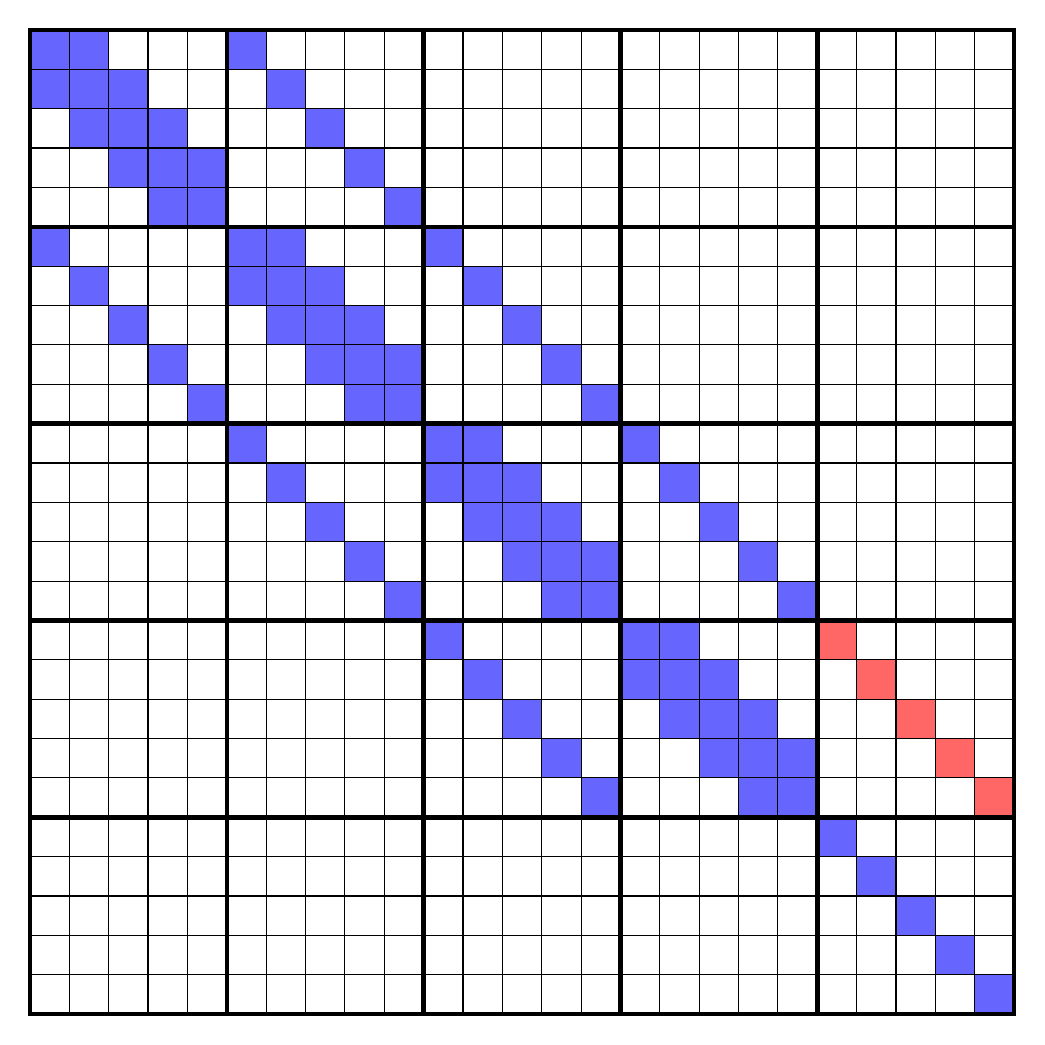
\begin{tikzpicture}[scale=0.5]

  % основная диагональ 
  \fill[color=blue!60] ( 0,24) rectangle ( 1,25);
  \fill[color=blue!60] ( 1,23) rectangle ( 2,24);
  \fill[color=blue!60] ( 2,22) rectangle ( 3,23);
  \fill[color=blue!60] ( 3,21) rectangle ( 4,22);
  \fill[color=blue!60] ( 4,20) rectangle ( 5,21);
  \fill[color=blue!60] ( 5,19) rectangle ( 6,20);
  \fill[color=blue!60] ( 6,18) rectangle ( 7,19);
  \fill[color=blue!60] ( 7,17) rectangle ( 8,18);
  \fill[color=blue!60] ( 8,16) rectangle ( 9,17);
  \fill[color=blue!60] ( 9,15) rectangle (10,16);
  \fill[color=blue!60] (10,14) rectangle (11,15);
  \fill[color=blue!60] (11,13) rectangle (12,14);
  \fill[color=blue!60] (12,12) rectangle (13,13);
  \fill[color=blue!60] (13,11) rectangle (14,12);
  \fill[color=blue!60] (14,10) rectangle (15,11);
  \fill[color=blue!60] (15, 9) rectangle (16,10);
  \fill[color=blue!60] (16, 8) rectangle (17, 9);
  \fill[color=blue!60] (17, 7) rectangle (18, 8);
  \fill[color=blue!60] (18, 6) rectangle (19, 7);
  \fill[color=blue!60] (19, 5) rectangle (20, 6);
  \fill[color=blue!60] (20, 4) rectangle (21, 5);
  \fill[color=blue!60] (21, 3) rectangle (22, 4);
  \fill[color=blue!60] (22, 2) rectangle (23, 3);
  \fill[color=blue!60] (23, 1) rectangle (24, 2);
  \fill[color=blue!60] (24, 0) rectangle (25, 1);
  

  % dow diag
  \fill[color=blue!60] ( 0,23) rectangle ( 1,24);
  \fill[color=blue!60] ( 1,22) rectangle ( 2,23);
  \fill[color=blue!60] ( 2,21) rectangle ( 3,22);
  \fill[color=blue!60] ( 3,20) rectangle ( 4,21);
  % \fill[color=blue!60] ( 4,19) rectangle ( 5,20);
  \fill[color=blue!60] ( 5,18) rectangle ( 6,19);
  \fill[color=blue!60] ( 6,17) rectangle ( 7,18);
  \fill[color=blue!60] ( 7,16) rectangle ( 8,17);
  \fill[color=blue!60] ( 8,15) rectangle ( 9,16);
  % \fill[color=blue!60] ( 9,14) rectangle (10,15);
  \fill[color=blue!60] (10,13) rectangle (11,14);
  \fill[color=blue!60] (11,12) rectangle (12,13);
  \fill[color=blue!60] (12,11) rectangle (13,12);
  \fill[color=blue!60] (13,10) rectangle (14,11);
  % \fill[color=blue!60] (14, 9) rectangle (15,10);
  \fill[color=blue!60] (15, 8) rectangle (16, 9);
  \fill[color=blue!60] (16, 7) rectangle (17, 8);
  \fill[color=blue!60] (17, 6) rectangle (18, 7);
  \fill[color=blue!60] (18, 5) rectangle (19, 6);
  % \fill[color=blue!60] (19, 4) rectangle (20, 5);
  % \fill[color=blue!60] (20, 3) rectangle (21, 4);
  % \fill[color=blue!60] (21, 2) rectangle (22, 3);
  % \fill[color=blue!60] (22, 1) rectangle (23, 2);
  % \fill[color=blue!60] (23, 0) rectangle (24, 1);


  % up diag    
  \fill[color=blue!60] ( 1,24) rectangle (2,25);
  \fill[color=blue!60] ( 2,23) rectangle ( 3,24);
  \fill[color=blue!60] ( 3,22) rectangle ( 4,23);
  \fill[color=blue!60] ( 4,21) rectangle ( 5,22);
  % \fill[color=blue!60] ( 5,20) rectangle ( 6,21);
  \fill[color=blue!60] ( 6,19) rectangle ( 7,20);
  \fill[color=blue!60] ( 7,18) rectangle ( 8,19);
  \fill[color=blue!60] ( 8,17) rectangle ( 9,18);
  \fill[color=blue!60] ( 9,16) rectangle (10,17);
  % \fill[color=blue!60] (10,15) rectangle (11,16);
  \fill[color=blue!60] (11,14) rectangle (12,15);
  \fill[color=blue!60] (12,13) rectangle (13,14);
  \fill[color=blue!60] (13,12) rectangle (14,13);
  \fill[color=blue!60] (14,11) rectangle (15,12);
  % \fill[color=blue!60] (15,10) rectangle (16,11);
  \fill[color=blue!60] (16, 9) rectangle (17,10);
  \fill[color=blue!60] (17, 8) rectangle (18, 9);
  \fill[color=blue!60] (18, 7) rectangle (19, 8);
  \fill[color=blue!60] (19, 6) rectangle (20, 7);
  % \fill[color=blue!60] (20, 5) rectangle (21, 6);
  % \fill[color=blue!60] (21, 4) rectangle (22, 5);
  % \fill[color=blue!60] (22, 3) rectangle (23, 4);
  % \fill[color=blue!60] (23, 2) rectangle (24, 3);
  % \fill[color=blue!60] (24, 1) rectangle (25, 2);

  % down diag

  \fill[color=blue!60] ( 0,19) rectangle ( 1,20);
  \fill[color=blue!60] ( 1,18) rectangle ( 2,19);
  \fill[color=blue!60] ( 2,17) rectangle ( 3,18);
  \fill[color=blue!60] ( 3,16) rectangle ( 4,17);
  \fill[color=blue!60] ( 4,15) rectangle ( 5,16);
  \fill[color=blue!60] ( 5,14) rectangle ( 6,15);
  \fill[color=blue!60] ( 6,13) rectangle ( 7,14);
  \fill[color=blue!60] ( 7,12) rectangle ( 8,13);
  \fill[color=blue!60] ( 8,11) rectangle ( 9,12);
  \fill[color=blue!60] ( 9,10) rectangle (10,11);
  \fill[color=blue!60] (10, 9) rectangle (11,10);
  \fill[color=blue!60] (11, 8) rectangle (12, 9);
  \fill[color=blue!60] (12, 7) rectangle (13, 8);
  \fill[color=blue!60] (13, 6) rectangle (14, 7);
  \fill[color=blue!60] (14, 5) rectangle (15, 6);
  % \fill[color=blue!60] (15, 4) rectangle (16, 5);
  % \fill[color=blue!60] (16, 3) rectangle (17, 4);
  % \fill[color=blue!60] (17, 2) rectangle (18, 3);
  % \fill[color=blue!60] (18, 1) rectangle (19, 2);
  % \fill[color=blue!60] (19, 0) rectangle (20, 1);

  % up diag

  \fill[color=blue!60] (5 ,24) rectangle (6 ,25);
  \fill[color=blue!60] (6 ,23) rectangle (7 ,24);
  \fill[color=blue!60] (7 ,22) rectangle (8 ,23);
  \fill[color=blue!60] (8 ,21) rectangle (9 ,22);
  \fill[color=blue!60] (9 ,20) rectangle (10,21);
  \fill[color=blue!60] (10,19) rectangle (11,20);
  \fill[color=blue!60] (11,18) rectangle (12,19);
  \fill[color=blue!60] (12,17) rectangle (13,18);
  \fill[color=blue!60] (13,16) rectangle (14,17);
  \fill[color=blue!60] (14,15) rectangle (15,16);
  \fill[color=blue!60] (15,14) rectangle (16,15);
  \fill[color=blue!60] (16,13) rectangle (17,14);
  \fill[color=blue!60] (17,12) rectangle (18,13);
  \fill[color=blue!60] (18,11) rectangle (19,12);
  \fill[color=blue!60] (19,10) rectangle (20,11);
  \fill[color=blue!60] (20, 9) rectangle (21,10);
  \fill[color=blue!60] (21, 8) rectangle (22, 9);
  \fill[color=blue!60] (22, 7) rectangle (23, 8);
  \fill[color=blue!60] (23, 6) rectangle (24, 7);
  \fill[color=blue!60] (24, 5) rectangle (25, 6);
  
  \fill[color=red!60] (20, 9) rectangle (21,10);
  \fill[color=red!60] (21, 8) rectangle (22, 9);
  \fill[color=red!60] (22, 7) rectangle (23, 8);
  \fill[color=red!60] (23, 6) rectangle (24, 7);
  \fill[color=red!60] (24, 5) rectangle (25, 6);
  
  % extra
  \draw[color=black,ultra thick] ( 5, 0) -- ( 5,25);
  \draw[color=black,ultra thick] (10, 0) -- (10,25);
  \draw[color=black,ultra thick] (15, 0) -- (15,25);
  \draw[color=black,ultra thick] (20, 0) -- (20,25);
  \draw[color=black,ultra thick] ( 0, 5) -- (25, 5);
  \draw[color=black,ultra thick] ( 0,10) -- (25,10);
  \draw[color=black,ultra thick] ( 0,15) -- (25,15);
  \draw[color=black,ultra thick] ( 0,20) -- (25,20);
  \draw[color=black,ultra thick] ( 0, 0) rectangle (25,25);
  
  \draw[color=black] ( 1, 0) -- ( 1,25);
  \draw[color=black] ( 6, 0) -- ( 6,25);
  \draw[color=black] (11, 0) -- (11,25);
  \draw[color=black] (16, 0) -- (16,25);
  \draw[color=black] (21, 0) -- (21,25);
  \draw[color=black] ( 2, 0) -- ( 2,25);
  \draw[color=black] ( 7, 0) -- ( 7,25);
  \draw[color=black] (12, 0) -- (12,25);
  \draw[color=black] (17, 0) -- (17,25);
  \draw[color=black] (22, 0) -- (22,25);
  \draw[color=black] ( 3, 0) -- ( 3,25);
  \draw[color=black] ( 8, 0) -- ( 8,25);
  \draw[color=black] (13, 0) -- (13,25);
  \draw[color=black] (18, 0) -- (18,25);
  \draw[color=black] (23, 0) -- (23,25);
  \draw[color=black] ( 4, 0) -- ( 4,25);
  \draw[color=black] ( 9, 0) -- ( 9,25);
  \draw[color=black] (14, 0) -- (14,25);
  \draw[color=black] (19, 0) -- (19,25);
  \draw[color=black] (24, 0) -- (24,25);
  
  \draw[color=black] ( 0, 1) -- (25, 1);
  \draw[color=black] ( 0, 6) -- (25, 6);
  \draw[color=black] ( 0,11) -- (25,11);
  \draw[color=black] ( 0,16) -- (25,16);
  \draw[color=black] ( 0,21) -- (25,21);
  \draw[color=black] ( 0, 2) -- (25, 2);
  \draw[color=black] ( 0, 7) -- (25, 7);
  \draw[color=black] ( 0,12) -- (25,12);
  \draw[color=black] ( 0,17) -- (25,17);
  \draw[color=black] ( 0,22) -- (25,22);
  \draw[color=black] ( 0, 3) -- (25, 3);
  \draw[color=black] ( 0, 8) -- (25, 8);
  \draw[color=black] ( 0,13) -- (25,13);
  \draw[color=black] ( 0,18) -- (25,18);
  \draw[color=black] ( 0,23) -- (25,23);
  \draw[color=black] ( 0, 4) -- (25, 4);
  \draw[color=black] ( 0, 9) -- (25, 9);
  \draw[color=black] ( 0,14) -- (25,14);
  \draw[color=black] ( 0,19) -- (25,19);
  \draw[color=black] ( 0,24) -- (25,24);
  \end{tikzpicture}
\end{figure}

\newpage
Уберем лишние элементы и получим систему с симметричной матрицей:

\begin{figure}[H]
  \centering
  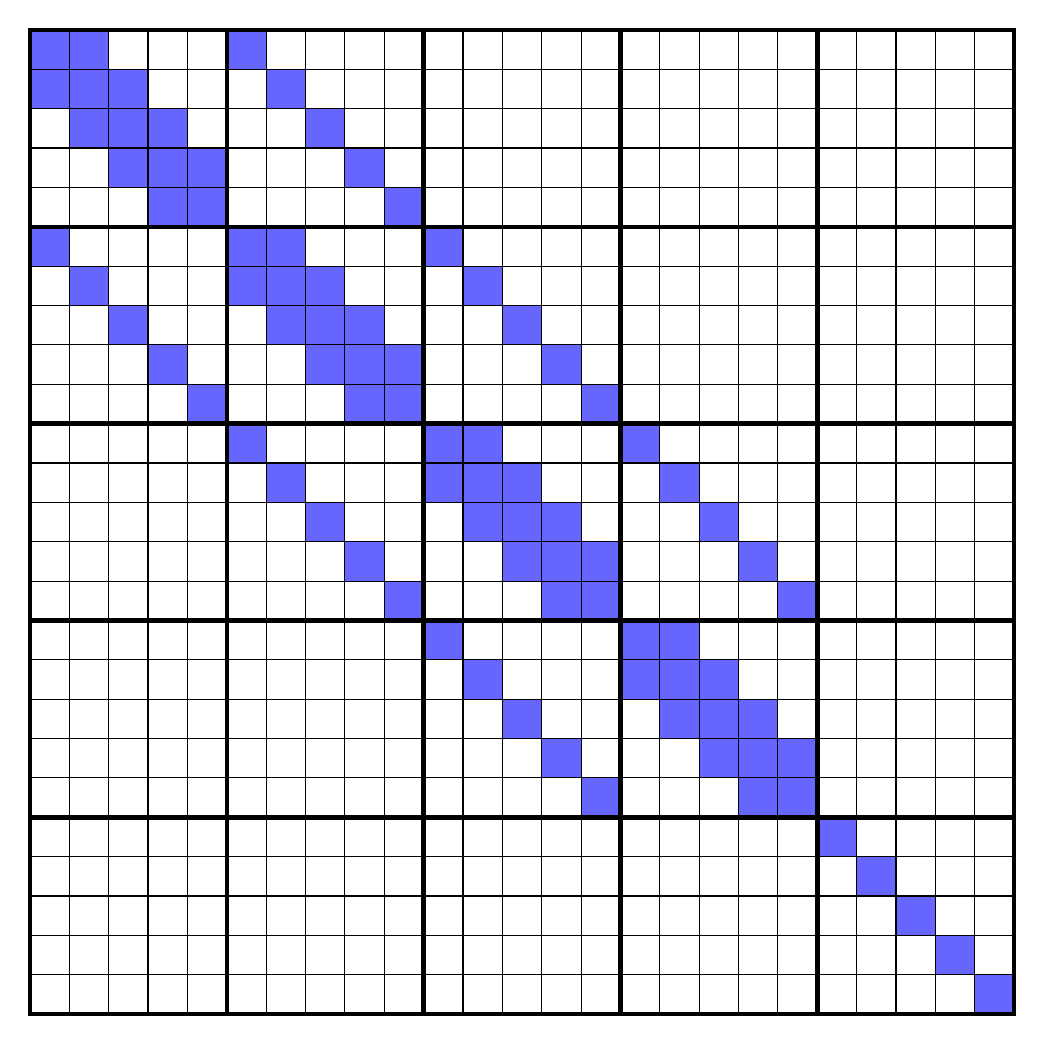
\begin{tikzpicture}[scale=0.5]

  % основная диагональ 
  \fill[color=blue!60] ( 0,24) rectangle ( 1,25);
  \fill[color=blue!60] ( 1,23) rectangle ( 2,24);
  \fill[color=blue!60] ( 2,22) rectangle ( 3,23);
  \fill[color=blue!60] ( 3,21) rectangle ( 4,22);
  \fill[color=blue!60] ( 4,20) rectangle ( 5,21);
  \fill[color=blue!60] ( 5,19) rectangle ( 6,20);
  \fill[color=blue!60] ( 6,18) rectangle ( 7,19);
  \fill[color=blue!60] ( 7,17) rectangle ( 8,18);
  \fill[color=blue!60] ( 8,16) rectangle ( 9,17);
  \fill[color=blue!60] ( 9,15) rectangle (10,16);
  \fill[color=blue!60] (10,14) rectangle (11,15);
  \fill[color=blue!60] (11,13) rectangle (12,14);
  \fill[color=blue!60] (12,12) rectangle (13,13);
  \fill[color=blue!60] (13,11) rectangle (14,12);
  \fill[color=blue!60] (14,10) rectangle (15,11);
  \fill[color=blue!60] (15, 9) rectangle (16,10);
  \fill[color=blue!60] (16, 8) rectangle (17, 9);
  \fill[color=blue!60] (17, 7) rectangle (18, 8);
  \fill[color=blue!60] (18, 6) rectangle (19, 7);
  \fill[color=blue!60] (19, 5) rectangle (20, 6);
  \fill[color=blue!60] (20, 4) rectangle (21, 5);
  \fill[color=blue!60] (21, 3) rectangle (22, 4);
  \fill[color=blue!60] (22, 2) rectangle (23, 3);
  \fill[color=blue!60] (23, 1) rectangle (24, 2);
  \fill[color=blue!60] (24, 0) rectangle (25, 1);
  

  % dow diag
  \fill[color=blue!60] ( 0,23) rectangle ( 1,24);
  \fill[color=blue!60] ( 1,22) rectangle ( 2,23);
  \fill[color=blue!60] ( 2,21) rectangle ( 3,22);
  \fill[color=blue!60] ( 3,20) rectangle ( 4,21);
  % \fill[color=blue!60] ( 4,19) rectangle ( 5,20);
  \fill[color=blue!60] ( 5,18) rectangle ( 6,19);
  \fill[color=blue!60] ( 6,17) rectangle ( 7,18);
  \fill[color=blue!60] ( 7,16) rectangle ( 8,17);
  \fill[color=blue!60] ( 8,15) rectangle ( 9,16);
  % \fill[color=blue!60] ( 9,14) rectangle (10,15);
  \fill[color=blue!60] (10,13) rectangle (11,14);
  \fill[color=blue!60] (11,12) rectangle (12,13);
  \fill[color=blue!60] (12,11) rectangle (13,12);
  \fill[color=blue!60] (13,10) rectangle (14,11);
  % \fill[color=blue!60] (14, 9) rectangle (15,10);
  \fill[color=blue!60] (15, 8) rectangle (16, 9);
  \fill[color=blue!60] (16, 7) rectangle (17, 8);
  \fill[color=blue!60] (17, 6) rectangle (18, 7);
  \fill[color=blue!60] (18, 5) rectangle (19, 6);
  % \fill[color=blue!60] (19, 4) rectangle (20, 5);
  % \fill[color=blue!60] (20, 3) rectangle (21, 4);
  % \fill[color=blue!60] (21, 2) rectangle (22, 3);
  % \fill[color=blue!60] (22, 1) rectangle (23, 2);
  % \fill[color=blue!60] (23, 0) rectangle (24, 1);


  % up diag    
  \fill[color=blue!60] ( 1,24) rectangle (2,25);
  \fill[color=blue!60] ( 2,23) rectangle ( 3,24);
  \fill[color=blue!60] ( 3,22) rectangle ( 4,23);
  \fill[color=blue!60] ( 4,21) rectangle ( 5,22);
  % \fill[color=blue!60] ( 5,20) rectangle ( 6,21);
  \fill[color=blue!60] ( 6,19) rectangle ( 7,20);
  \fill[color=blue!60] ( 7,18) rectangle ( 8,19);
  \fill[color=blue!60] ( 8,17) rectangle ( 9,18);
  \fill[color=blue!60] ( 9,16) rectangle (10,17);
  % \fill[color=blue!60] (10,15) rectangle (11,16);
  \fill[color=blue!60] (11,14) rectangle (12,15);
  \fill[color=blue!60] (12,13) rectangle (13,14);
  \fill[color=blue!60] (13,12) rectangle (14,13);
  \fill[color=blue!60] (14,11) rectangle (15,12);
  % \fill[color=blue!60] (15,10) rectangle (16,11);
  \fill[color=blue!60] (16, 9) rectangle (17,10);
  \fill[color=blue!60] (17, 8) rectangle (18, 9);
  \fill[color=blue!60] (18, 7) rectangle (19, 8);
  \fill[color=blue!60] (19, 6) rectangle (20, 7);
  % \fill[color=blue!60] (20, 5) rectangle (21, 6);
  % \fill[color=blue!60] (21, 4) rectangle (22, 5);
  % \fill[color=blue!60] (22, 3) rectangle (23, 4);
  % \fill[color=blue!60] (23, 2) rectangle (24, 3);
  % \fill[color=blue!60] (24, 1) rectangle (25, 2);

  % down diag

  \fill[color=blue!60] ( 0,19) rectangle ( 1,20);
  \fill[color=blue!60] ( 1,18) rectangle ( 2,19);
  \fill[color=blue!60] ( 2,17) rectangle ( 3,18);
  \fill[color=blue!60] ( 3,16) rectangle ( 4,17);
  \fill[color=blue!60] ( 4,15) rectangle ( 5,16);
  \fill[color=blue!60] ( 5,14) rectangle ( 6,15);
  \fill[color=blue!60] ( 6,13) rectangle ( 7,14);
  \fill[color=blue!60] ( 7,12) rectangle ( 8,13);
  \fill[color=blue!60] ( 8,11) rectangle ( 9,12);
  \fill[color=blue!60] ( 9,10) rectangle (10,11);
  \fill[color=blue!60] (10, 9) rectangle (11,10);
  \fill[color=blue!60] (11, 8) rectangle (12, 9);
  \fill[color=blue!60] (12, 7) rectangle (13, 8);
  \fill[color=blue!60] (13, 6) rectangle (14, 7);
  \fill[color=blue!60] (14, 5) rectangle (15, 6);
  % \fill[color=blue!60] (15, 4) rectangle (16, 5);
  % \fill[color=blue!60] (16, 3) rectangle (17, 4);
  % \fill[color=blue!60] (17, 2) rectangle (18, 3);
  % \fill[color=blue!60] (18, 1) rectangle (19, 2);
  % \fill[color=blue!60] (19, 0) rectangle (20, 1);

  % up diag

  \fill[color=blue!60] (5 ,24) rectangle (6 ,25);
  \fill[color=blue!60] (6 ,23) rectangle (7 ,24);
  \fill[color=blue!60] (7 ,22) rectangle (8 ,23);
  \fill[color=blue!60] (8 ,21) rectangle (9 ,22);
  \fill[color=blue!60] (9 ,20) rectangle (10,21);
  \fill[color=blue!60] (10,19) rectangle (11,20);
  \fill[color=blue!60] (11,18) rectangle (12,19);
  \fill[color=blue!60] (12,17) rectangle (13,18);
  \fill[color=blue!60] (13,16) rectangle (14,17);
  \fill[color=blue!60] (14,15) rectangle (15,16);
  \fill[color=blue!60] (15,14) rectangle (16,15);
  \fill[color=blue!60] (16,13) rectangle (17,14);
  \fill[color=blue!60] (17,12) rectangle (18,13);
  \fill[color=blue!60] (18,11) rectangle (19,12);
  \fill[color=blue!60] (19,10) rectangle (20,11);
  % \fill[color=blue!60] (20, 9) rectangle (21,10);
  % \fill[color=blue!60] (21, 8) rectangle (22, 9);
  % \fill[color=blue!60] (22, 7) rectangle (23, 8);
  % \fill[color=blue!60] (23, 6) rectangle (24, 7);
  % \fill[color=blue!60] (24, 5) rectangle (25, 6);
  
  % \fill[color=red!60] (20, 9) rectangle (21,10);
  % \fill[color=red!60] (21, 8) rectangle (22, 9);
  % \fill[color=red!60] (22, 7) rectangle (23, 8);
  % \fill[color=red!60] (23, 6) rectangle (24, 7);
  % \fill[color=red!60] (24, 5) rectangle (25, 6);
  
  % extra
  \draw[color=black,ultra thick] ( 5, 0) -- ( 5,25);
  \draw[color=black,ultra thick] (10, 0) -- (10,25);
  \draw[color=black,ultra thick] (15, 0) -- (15,25);
  \draw[color=black,ultra thick] (20, 0) -- (20,25);
  \draw[color=black,ultra thick] ( 0, 5) -- (25, 5);
  \draw[color=black,ultra thick] ( 0,10) -- (25,10);
  \draw[color=black,ultra thick] ( 0,15) -- (25,15);
  \draw[color=black,ultra thick] ( 0,20) -- (25,20);
  \draw[color=black,ultra thick] ( 0, 0) rectangle (25,25);
  
  \draw[color=black] ( 1, 0) -- ( 1,25);
  \draw[color=black] ( 6, 0) -- ( 6,25);
  \draw[color=black] (11, 0) -- (11,25);
  \draw[color=black] (16, 0) -- (16,25);
  \draw[color=black] (21, 0) -- (21,25);
  \draw[color=black] ( 2, 0) -- ( 2,25);
  \draw[color=black] ( 7, 0) -- ( 7,25);
  \draw[color=black] (12, 0) -- (12,25);
  \draw[color=black] (17, 0) -- (17,25);
  \draw[color=black] (22, 0) -- (22,25);
  \draw[color=black] ( 3, 0) -- ( 3,25);
  \draw[color=black] ( 8, 0) -- ( 8,25);
  \draw[color=black] (13, 0) -- (13,25);
  \draw[color=black] (18, 0) -- (18,25);
  \draw[color=black] (23, 0) -- (23,25);
  \draw[color=black] ( 4, 0) -- ( 4,25);
  \draw[color=black] ( 9, 0) -- ( 9,25);
  \draw[color=black] (14, 0) -- (14,25);
  \draw[color=black] (19, 0) -- (19,25);
  \draw[color=black] (24, 0) -- (24,25);
  
  \draw[color=black] ( 0, 1) -- (25, 1);
  \draw[color=black] ( 0, 6) -- (25, 6);
  \draw[color=black] ( 0,11) -- (25,11);
  \draw[color=black] ( 0,16) -- (25,16);
  \draw[color=black] ( 0,21) -- (25,21);
  \draw[color=black] ( 0, 2) -- (25, 2);
  \draw[color=black] ( 0, 7) -- (25, 7);
  \draw[color=black] ( 0,12) -- (25,12);
  \draw[color=black] ( 0,17) -- (25,17);
  \draw[color=black] ( 0,22) -- (25,22);
  \draw[color=black] ( 0, 3) -- (25, 3);
  \draw[color=black] ( 0, 8) -- (25, 8);
  \draw[color=black] ( 0,13) -- (25,13);
  \draw[color=black] ( 0,18) -- (25,18);
  \draw[color=black] ( 0,23) -- (25,23);
  \draw[color=black] ( 0, 4) -- (25, 4);
  \draw[color=black] ( 0, 9) -- (25, 9);
  \draw[color=black] ( 0,14) -- (25,14);
  \draw[color=black] ( 0,19) -- (25,19);
  \draw[color=black] ( 0,24) -- (25,24);
  \end{tikzpicture}
\end{figure}

Данную систему мы будем решать методом сопряжённых градиентов.
